%%%%%%%%%%%%%%%%%%%%%%%%%% template.tex %%%%%%%%%%%%%%%%%%%%%%%%%%%
%
% sample input file for your contribution to Springer ENCYCLOPEDIAs
%
% Use this file as a template for your own input.
%
%%%%%%%%%%%%%%%%%%%%%%%% Springer-Verlag %%%%%%%%%%%%%%%%%%%%%%%%%%


% RECOMMENDED %%%%%%%%%%%%%%%%%%%%%%%%%%%%%%%%%%%%%%%%%%%%%%%%%%%%%
\documentclass{svcyclop}

% \documentclass[natbib]{svcyclop}
% call for the natbib-system if you wish to have sophisticated citations,
% remember to adapt the references at the end of your contribution then
% see explanation at the end of this file.
%
% A detailed explanation and demonstration of the natbib system can
% be found at
%     http://merkel.zoneo.net/Latex/natbib.php
%
% If you use BibTeX to manage your citation use the style "spbasic.bst"
% that is "natbib" aware.

\usepackage{graphicx}    % standard LaTeX graphics tool
                         % when including figure files

% \usepackage{amsfonts,amsmath} % useful for typesetting complicated math

% Hint:
% Use the "hyperref" package in the preamble
% if you want to supply active links within
% your text; e.g. at the \CrossRef section
% \usepackage{hyperref}

% Hint:
% Use the package "url" in the preamble
% to avoid problems with special characters
% used in your e-mail or web address in the
% \author or the \institute field below
% \usepackage{url}
% \urlstyle{tt}    % URLs are typeset in typewriter font

% etc.

%%%%%%%%%%%%%%%%%%%%%%%%%%%%%%%%%%%%%%%%%%%%%%%%%%%%%%%%%%%%%%%%%%%

\begin{document}

% Please specify your Entry Title in one continuous line
\title{}

% Please specify the Names of Entry Author(s)
\author{}
% if there is more than one author, use "\and" in between
% the particular author lines
%
% add "\inst{<No.>}" directly after the author name to indicate
% the mapping to the relevant affiliations/addresses in the
% forthcoming "\institute" field
%
% see also the example contribution file "example.tex" for detailed info

% Please specify your Address/Affiliation and use "\\" as EOL for structuring
% specify Phone / Fax / e-mail if applicable, use "\\" as EOL for structuring
% more than one address/affiliation? separate each two entries with
% a line containing "\and"
\institute{}
% make sure to give at least as many institute addresses
% as the mapping to the authors requires;
% the numbering is done automatically by the "\and" command
% see also the example contribution file "example.tex" for detailed info

% Please specify Years and Authors of Summarized Original Work
% use one continuous line for each paper; use semicolon to separate
% the year from the last names; don't use "and" between author names
% adhere to the following format:
% "Year of paper"; "last names of authors" separated by commas without "and"
% use "\\" as EOL for structuring
\sumoriwork{}
% see also the example contribution file "example.tex"
% for detailed information
%

% Please specify the Keywords - use semicolon for separation
\keywords{}

\maketitle  % completes, checks, and typesets the contribution's head

% you have 7 predefined headings at hand you can use throughout your contribution;
% just call the relevant commands instead of generating a new "\section" for them;
% the next two headings are mandatory:
% \ProbDef   -   Problem Definition
% \KeyRes    -   Key Results
%
% the following heading commands may be used as and when required:
% \Applic    -   Applications
% \OpenProb  -   Open Problems
% \ExpRes    -   Experimental Results
% \DataSets  -   URLs to Code and Data Sets
% \CrossRef  -   Cross References

\section{Section Heading}
Your text comes here.

\subsection{Subsection Heading}
Your text comes here.

\subsubsection{Subsubsection Heading}
Your text comes here.

\paragraph{Paragraph Heading} as required
Your text comes here.
%
% For tables use
%
\begin{table}
\caption{Please write your table caption here}
\label{tab:1}       % Give a unique label
% For LaTeX tables use
\begin{tabular}{lll}
\hline\noalign{\smallskip}
first & second & third  \\
\noalign{\smallskip}\hline\noalign{\smallskip}
number & number & number \\
number & number & number \\
\noalign{\smallskip}\hline
\end{tabular}
\end{table}
%
% For figures use
%
\begin{figure}
\centering
% Use the relevant command for your figure-insertion program
% to insert the figure file.
% For example, with the option graphics use
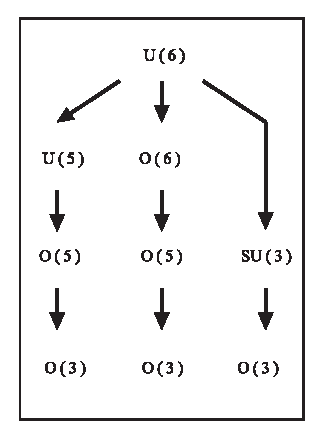
\includegraphics[height=4cm]{figure}
% If not, use
%\mpicplace{5cm}{2cm} % Give the correct figure height and width in cm
\caption{Please write your figure caption here}
\label{fig:1}       % Give a unique label
\end{figure}
%
% BibTeX users please use
% \bibliographystyle{spbasic}
% \bibliography{mydatabase}
%
% Non-BibTeX users please use
\begin{thebibliography}{8.}
%
% and use \bibitem to create references.
%
% Use the following syntax and markup for your references
%
% Complete Book
\bibitem{book} Faber K (1997) Biotransformations in organic
chemistry, 3rd edn. Springer, Berlin Heidelberg New York

% Contributions, Chapters or Sections in Books
\bibitem{contribution} Brown FR, Jackson D (1987) Analytical chemistry.
In: Whie FC, Red SA (eds) Modern chemistry. Springer, Berlin Heidelberg
New York, p 220

% Journal
\bibitem{journal}
Fuchigami T (1994) Top Curr Chem 170:25

% Other Possibilities
\bibitem{Other} Tanzawa H (1986) First Japan-US workshop on Biomedical
Polymer Science. Kyoto, Japan

\end{thebibliography}

%%%%%%%%%%%%%%%%%%%%%%%%%%%%%%%%%%%%%%%%%%%%%%%%%%%%%%%%%%%%%%%%%%%%%%

\end{document}

% here a faked reference section follows working with the natbib-system
% allowing for author-year citation without automated BibTeX usage

% Non-BibTeX users please use
\begin{thebibliography}{99}
%
% and use \bibitem to create references. Consult the Instructions
% for authors for reference list style.
%
% Format for Journal Reference
\bibitem[Author I(1999)]{RefJ}
Author I (year) Article title. Journal Title-Abbreviated Vol: pp--pp

\bibitem[{{Daiguji} et~al(2004){Daiguji}, {Yang}, {Szeri} and
{Majumdar}}]{daiyaszma04}
{Daiguji} H, {Yang} PD, {Szeri} AJ, and {Majumdar} A (2004)
Electrochemomechanical energy conversion in nanofluidic channels. Nano
Letters 4 (12): 2315-2321.

% Format for books
\bibitem[Author and Smith(2001)]{RefB}
Author I, Smith J (year) Book title. Publisher, Place, pp numbers

\bibitem[{{Dukhin} et~al(1974){Dukhin} and {Deryaguin}}]{dukhin74}
{Dukhin} SS and {Deryaguin} BV {({1974})} {Electro-kinetic phenomena}
In: Matijevic E (ed) Surface and Colloid Science. John Wiley, New York.
% etc
\end{thebibliography}

\end{document}
% end of file "template.tex"
